\section{eo\-Fitness\-Scaling\-Select$<$ EOT $>$ Class Template Reference}
\label{classeo_fitness_scaling_select}\index{eoFitnessScalingSelect@{eoFitnessScalingSelect}}
eo\-Fitness\-Scaling\-Select: select an individual proportional to the linearly scaled fitness that is computed by the private {\bf eo\-Linear\-Fit\-Scaling}{\rm (p.\,\pageref{classeo_linear_fit_scaling})} object  


{\tt \#include $<$eo\-Fitness\-Scaling\-Select.h$>$}

Inheritance diagram for eo\-Fitness\-Scaling\-Select$<$ EOT $>$::\begin{figure}[H]
\begin{center}
\leavevmode
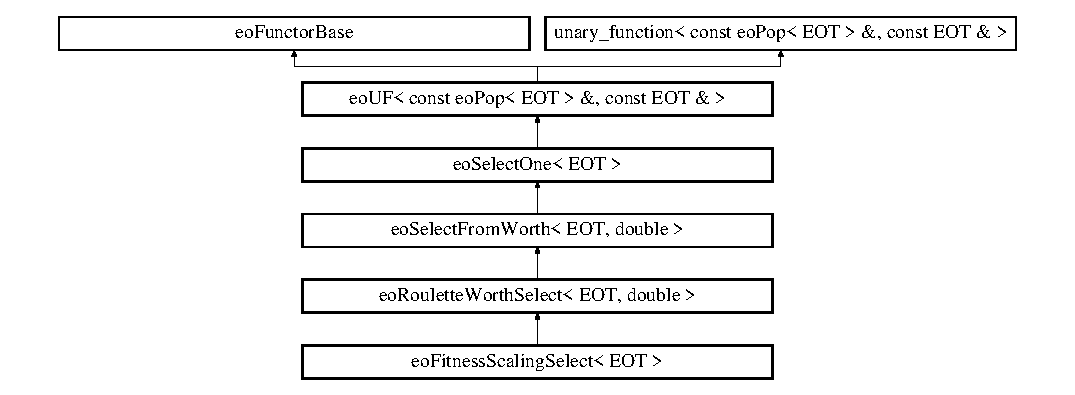
\includegraphics[height=4.85549cm]{classeo_fitness_scaling_select}
\end{center}
\end{figure}
\subsection*{Public Member Functions}
\begin{CompactItemize}
\item 
{\bf eo\-Fitness\-Scaling\-Select} (double \_\-p=2.0)
\begin{CompactList}\small\item\em Ctor:. \item\end{CompactList}\end{CompactItemize}
\subsection*{Private Attributes}
\begin{CompactItemize}
\item 
{\bf eo\-Linear\-Fit\-Scaling}$<$ {\bf EOT} $>$ {\bf scaling}\label{classeo_fitness_scaling_select_r0}

\end{CompactItemize}


\subsection{Detailed Description}
\subsubsection*{template$<$class EOT$>$ class eo\-Fitness\-Scaling\-Select$<$ EOT $>$}

eo\-Fitness\-Scaling\-Select: select an individual proportional to the linearly scaled fitness that is computed by the private {\bf eo\-Linear\-Fit\-Scaling}{\rm (p.\,\pageref{classeo_linear_fit_scaling})} object 



Definition at line 40 of file eo\-Fitness\-Scaling\-Select.h.

\subsection{Constructor \& Destructor Documentation}
\index{eoFitnessScalingSelect@{eo\-Fitness\-Scaling\-Select}!eoFitnessScalingSelect@{eoFitnessScalingSelect}}
\index{eoFitnessScalingSelect@{eoFitnessScalingSelect}!eoFitnessScalingSelect@{eo\-Fitness\-Scaling\-Select}}
\subsubsection{\setlength{\rightskip}{0pt plus 5cm}template$<$class EOT$>$ {\bf eo\-Fitness\-Scaling\-Select}$<$ {\bf EOT} $>$::{\bf eo\-Fitness\-Scaling\-Select} (double {\em \_\-p} = {\tt 2.0})\hspace{0.3cm}{\tt  [inline]}}\label{classeo_fitness_scaling_select_a0}


Ctor:. 

\begin{Desc}
\item[Parameters:]
\begin{description}
\item[{\em \_\-p}]the selective pressure, should be in [1,2] (2 is the default) \end{description}
\end{Desc}


Definition at line 46 of file eo\-Fitness\-Scaling\-Select.h.

The documentation for this class was generated from the following file:\begin{CompactItemize}
\item 
eo\-Fitness\-Scaling\-Select.h\end{CompactItemize}
